\documentclass{article}

\usepackage{tikz}
\usepackage{listings}
\usepackage{csvsimple}

\begin{document}

\section{Body}
One of the first models of drone behavior we thought of is that drones fly
	in straight lines, and do not interact with other drones.
When a drone reaches the boundary of the surveillance region, that drone
	``bounces off'' (see Figure \ref{fig:drone-barrier-bounce}).
Note that if the wall is vertical, the bouncing just multiplies the $x$
	component of the velocity by $-1$.

\begin{figure}[h]
\begin{center}
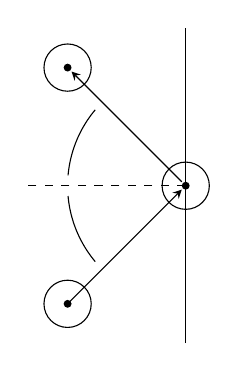
\begin{tikzpicture}

% wall/boundary for drone to bounce off of
\draw (1,-2) to (1,2);

% drone before bounce
\draw (-0.5,-1.5) circle (0.3);
\fill (-0.5,-1.5) circle [radius=0.05];

% drone during bounce
\draw (1.0, 0.0) circle (0.3);
\fill (1.0, 0.0) circle [radius=0.05];

% drone after bounce
\draw (-0.5, 1.5) circle (0.3);
\fill (-0.5, 1.5) circle (0.05);

% bouncing arrows
\draw[->,>=stealth] (-0.5, -1.5) -- (0.95,-0.05);
\draw[->,>=stealth] (0.95, 0.05) -- (-0.45, 1.45);

% line of symmetry
\draw[dashed] (1,0) to (-1,0);

% angle measures
\draw[domain=140:175] plot ({1 + 1.5*cos(\x)}, {1.5*sin(\x)});
\draw[domain=-175:-140] plot ({1 + 1.5*cos(\x)}, {1.5*sin(\x)});

\end{tikzpicture}
\end{center}
\caption{An incoming drone bounces off of a barrier.  The circle is its radius
	of vision.}
\label{fig:drone-barrier-bounce}
\end{figure}


If the drones do not interact with each other, and are given uniformly random
	velocities and positions, then they should be distributed uniformly throughout
	the surveillence domain.

We have implemented a simulation of this model in matlab.
A typical moment in time looks like this:

\begin{figure}[h]
\begin{center}
\begin{tikzpicture}
\end{tikzpicture}
\end{center}
\end{figure}

Notice that in this case, the drones' fields of view are overlapping.

\section{Code Appendix}
\lstinputlisting[language=octave,
	caption={Ideal Gas Simulation}, 
	label=code:ideal-gas]
{ideal-gas.m}

\end{document}
